\section{Lottery scheduling}
Lottery scheduling es un algoritmo de planificaci\'on probabilistico para los procesos de un sistema operativo. A cada proceso se les asigna un n\'umero de billetes de loter\'ia, y se elije un boleto al azar para seleccionar el siguiente proceso. La distribución de los billetes no tiene por qu\'e ser uniforme, darle más billetes a un proceso le ofrece una oportunidad mayor de salir seleccionado.

\subsection{Implementaci\'on propuesta}
A la hora de implementar este algoritmo, recurrimos al paper de Waldspurger y Weihl, \textit{Lottery scheduling: Flexible proportional - share resource management} el cual explica los detalles del algoritmo. 

En dicho paper, adem\'as del sistema de tickets se propone un sistema de monedas o \textit{currencies} las cuales respaldan los tickets. El sistema cuenta con una moneda base que respalda una serie de tickets repartidos entre los usuarios que lanzan los procesos. A su vez, cada usuario emite una moneda para respaldar los tickets que reciben sus procesos. Lo mismo sucede con los procesos y sus \textit{threads}. Como en el simulador provisto por la c\'atedra no existen los usuarios ni los \textit{threads}, implementamos \'unicamente el sistema de tickets base.

A continuaci\'on explicaremos los pasos de nuestra implementacion que utiliza los mismos m\'etodos que la vista para Round Robin.

\begin{itemize}
	\item El método \textit{load(pid)} se agrega a nuestro diccionario de tareas el nuevo \textit{pid} y se le da un ticket.
	\item El método \textit{unblock(pid)} se la desmarca como bloqueada.
	\item El método \textit{tick(motivo)} se ejecuta por cada tick del reloj de la máquina el simulador. El parámetro \textbf{motivo} indica lo que ocurrió con la tarea que ocupaba el CPU el ciclo de reloj anterior:
	
	\begin{itemize}
		\item Si el \textbf{motivo} es \textit{exit}: se saca la tarea de nuestro diccionario y se hace un nuevo sorteo.
		\item Si el \textbf{motivo} es \textit{block}: se la demarca como bloqueada y se la compensa con $\frac{quantum}{quantum - f}$ donde \textit{f} es la fracci\'on de \textit{quantum} que utiliz\'o.
		\item Si el \textbf{motivo} es \textit{tick}: si se termina el \textit{quantum} de esa tarea, se la desaloja y se realiza un sorteo. La nueva tarea elegida es puesta a trabajar y se le deja un solo ticket. Si no hay m\'as tareas o est\'an todas bloqueadas, trabaja la \verb|idle_task|.
	\end{itemize}
\end{itemize}

\subsection{Diagrama de estados}
\begin{center}
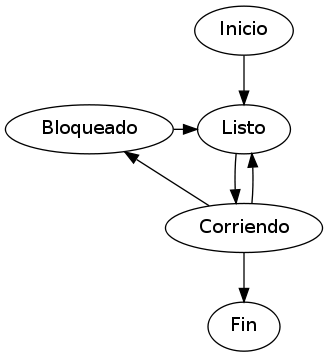
\includegraphics[scale=0.5]{estados.png}
\end{center}

\subsection{An\'alisis del algoritmo}
\begin{figure}[H]
\centering
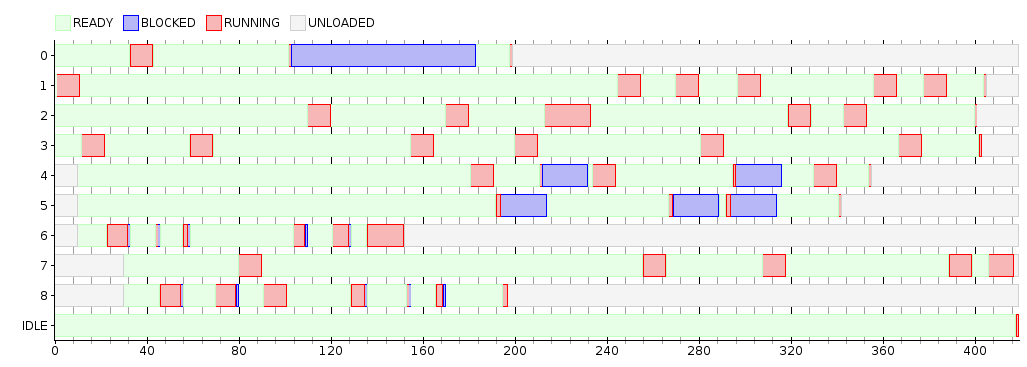
\includegraphics[scale=0.5]{./graficos/out_ej_8.png}
\caption{Lottery - Quantum 10, Semilla 1315772865}
\end{figure} 

\begin{figure}[H]
\centering
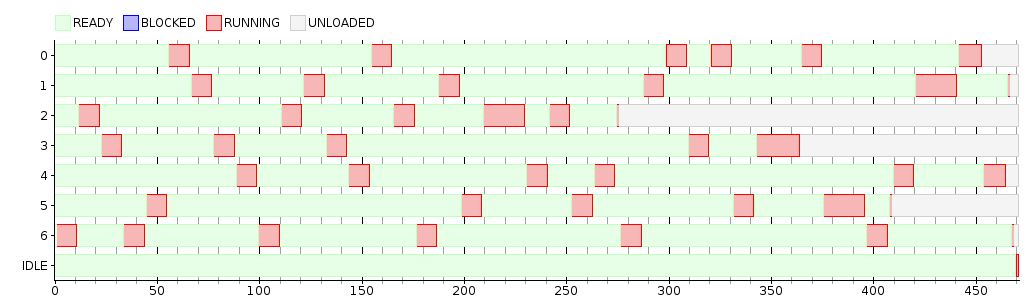
\includegraphics[scale=0.5]{./graficos/out_ej_8_2.png}
\caption{Lottery - Quantum 10, Semilla 1315772865}
\end{figure} 

\begin{figure}[H]
\centering
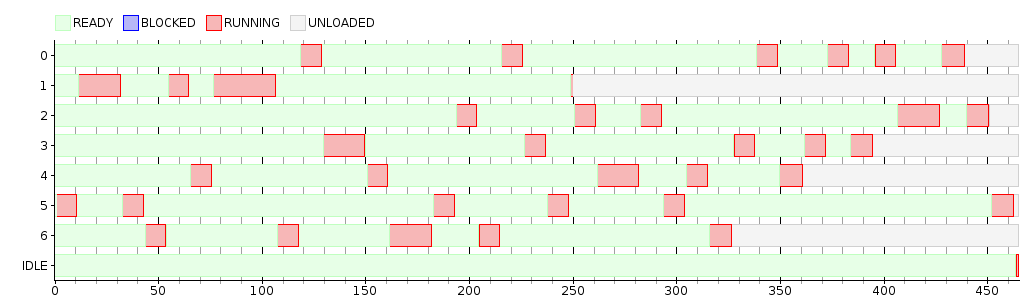
\includegraphics[scale=0.5]{./graficos/out_ej_8_3.png}
\caption{Lottery - Quantum 10, Semilla 1315793579}
\end{figure} 

